\indent Veremos que es lo que sucede al ir variando los parámetros de entrada para cada familia, de manera tal que, a medida que F, C y P crecen linealmente podamos observar que sucede con cada familia de casos (es decir, las familias se mantienen, solo varia el tamaño de la entrada en todos los casos).\\
Se comienza, por lo tanto, con una entrada de 5 filas y columnas y se la aumenta en cada test en una fila y columna hasta llegar a una matriz de 50*50. De manera que no hay desigualdades y todas las familias se miden en instancias de igual tamaño.\\
El origen siempre estará en la primer columna posible y el destino en la última. A medida que la matriz crezca, las posiciones de los mismos no serán alteradas y la cantidad de paredes y como varie el $P_{max}$ en cada caso, serán acordes para que siempre se encuentren dentro de la misma familia.

Para obtener dichas instancias se realizaron aproximadamente unas 20 corridas con el mismo input y se tom\'o el promedio de las mismas en cada instancia para obtener un valor m\'as cercano a la media.\\ 



Se puede observar en el  gráfico 1.1, cinco funciones, que representan el tiempo de ejecuci\'on de las familias de casos mencionadas en el apartado anterior:\\

\begin{enumerate}
\item No existe camino para atravezar el laberinto
\item Existe un camino sin atravesar paredes para recorrer todo el laberinto
\item Rompiendo todas las paredes posibles para pasar el laberinto
\item Rompiendo una cantidad menor de paredes posibles para pasar el laberinto
\item Múltiples caminos para llegar a destino
\end{enumerate}

\vspace*{0.3cm} \vspace*{0.3cm}
  \begin{center}
 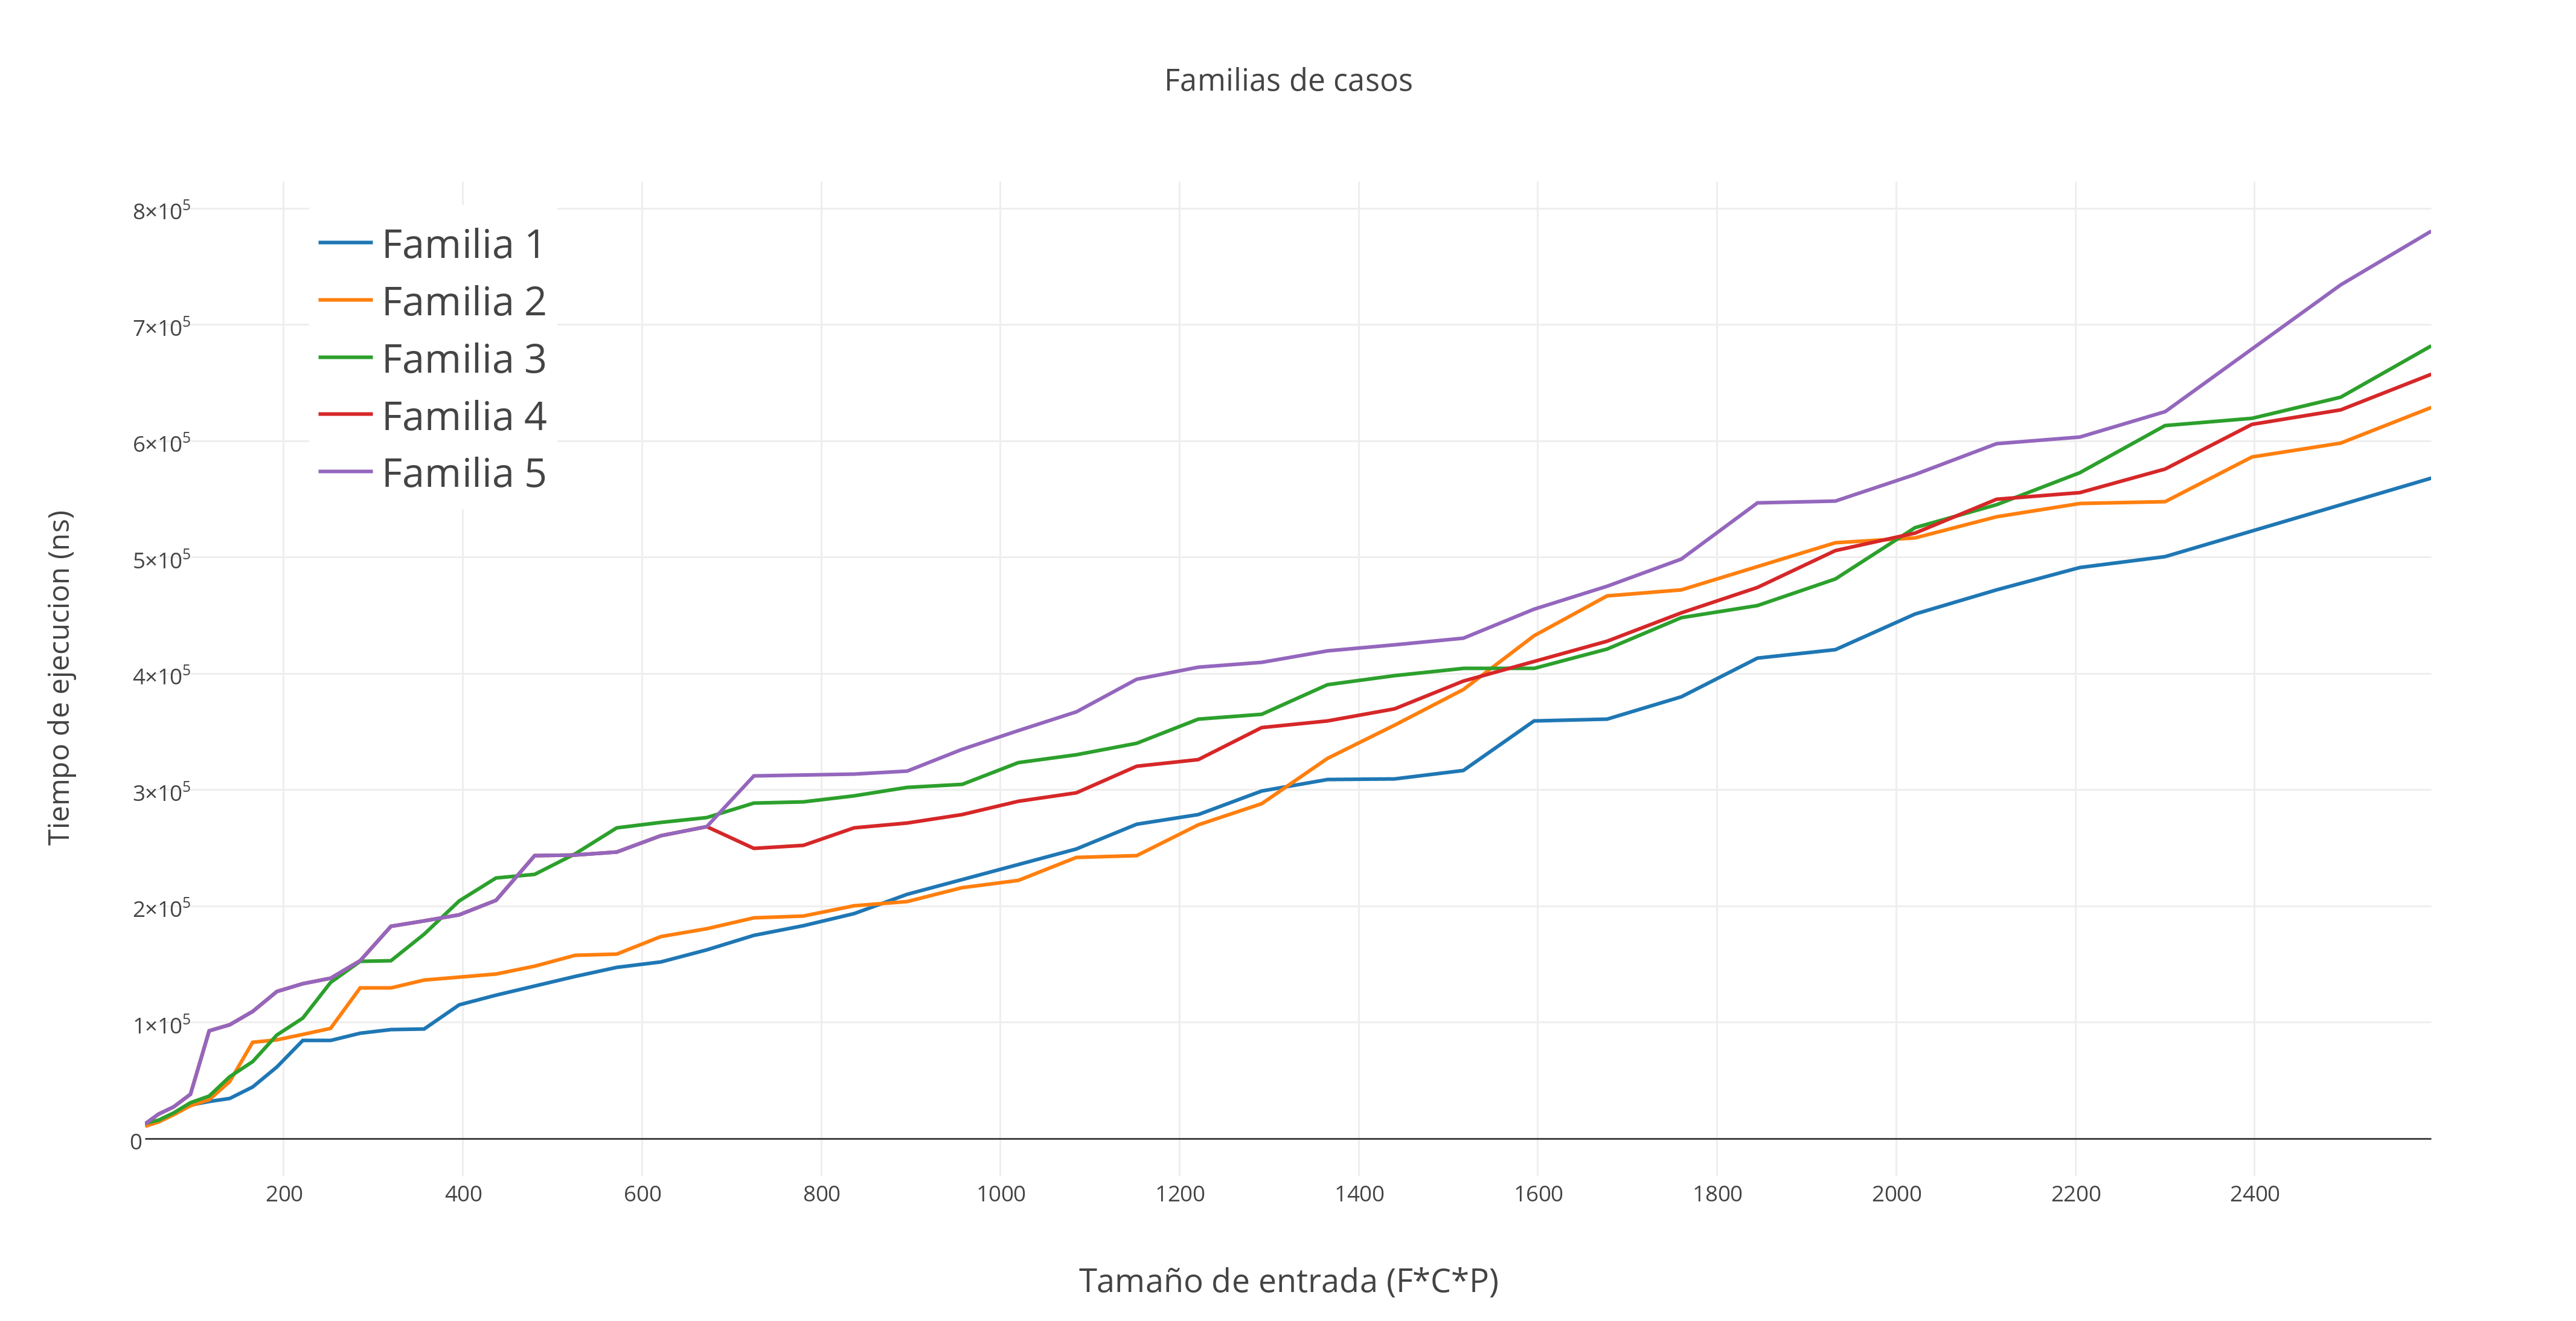
\includegraphics[scale=0.5]{./EJ1/comparativo.png}
 {Gr\'afico \ 1.1 - $Comparativo$}
  \end{center}
  \vspace*{0.3cm}
  
Se puede notar que la familia 1 "\textbf{No existe camino para atravezar el laberinto}", presenta una mejor performance en relaci\'on a las otras. Esto se puede deber a dos motivos, o bien en el primer paso no puede salir por ning\'un camino posible o bien su adyacente es el nodo destino, por lo tanto chequea solo los nodos adyacentes al origen y finaliza su ejecuci\'on. Con lo cual esta familia representa el mejor caso en performance para el algoritmo.

\vspace*{0.3cm} \vspace*{0.3cm}
  \begin{center}
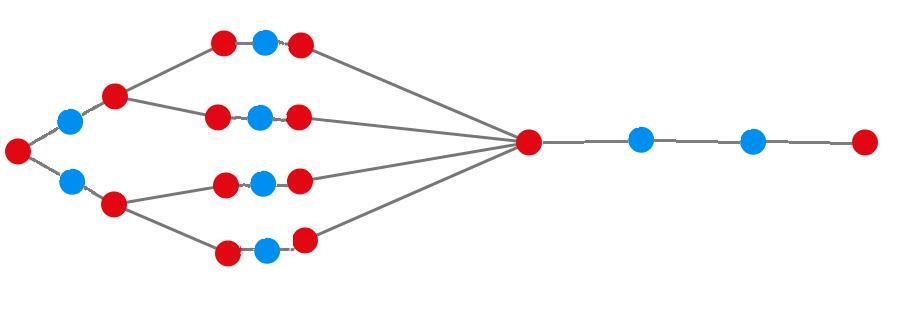
\includegraphics[scale=0.7]{./EJ1/ej1grafomejorcaso.jpeg}
{Grafo 1.1 - $Con$ $P=0$ Termina sin poder romper paredes en una iteracion}
  \end{center}
  \vspace*{0.3cm}

\vspace*{0.3cm} \vspace*{0.3cm}
  \begin{center}
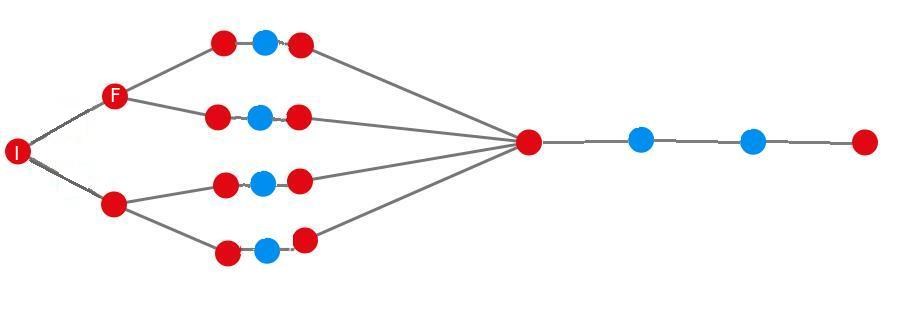
\includegraphics[scale=0.7]{./EJ1/ej1grafomejorcaso2.jpeg}
{Grafo 1.1 - $Con$ $P=0$ Nodo destino (f) vecino a nodo inicio (i)}
  \end{center}
  \vspace*{0.3cm}

Uno de los peores casos para nuestro algoritmo es la familia 5 "\textbf{Múltiples caminos para llegar a destino}", que sucede cuando por ejemplo, todos los caminos tienen igual longitud. Esto se da as\'i ya que nuestro algoritmo chequea todos los caminos posibles y como todos pueden ser soluci\'on posible avanza por todos y llega al final del laberinto con el mismo valor en todos los posibles caminos.\\

\vspace*{0.3cm} \vspace*{0.3cm}
  \begin{center}
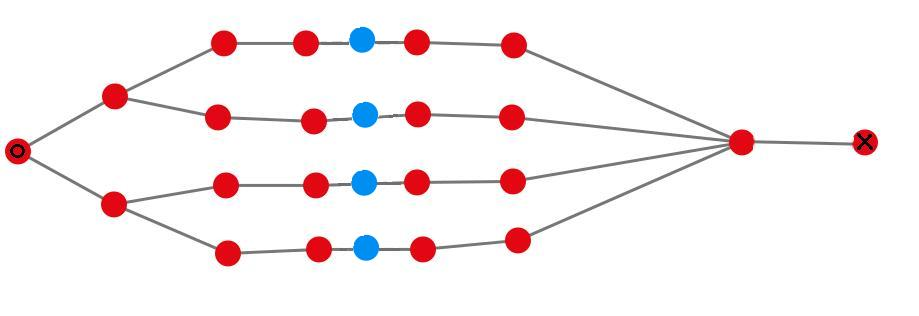
\includegraphics[scale=0.7]{./EJ1/ej1grafopeorcaso.jpeg}
{Gr\'afico 1.2 - Múltiples caminos para llegar a destino de misma longitud}
  \end{center}
  \vspace*{0.3cm}

Veamos en detalle como se comportan el mejor y peor caso con respecto a la complejidad calculada.\\

  \vspace*{0.3cm} \vspace*{0.3cm}
  \begin{center}
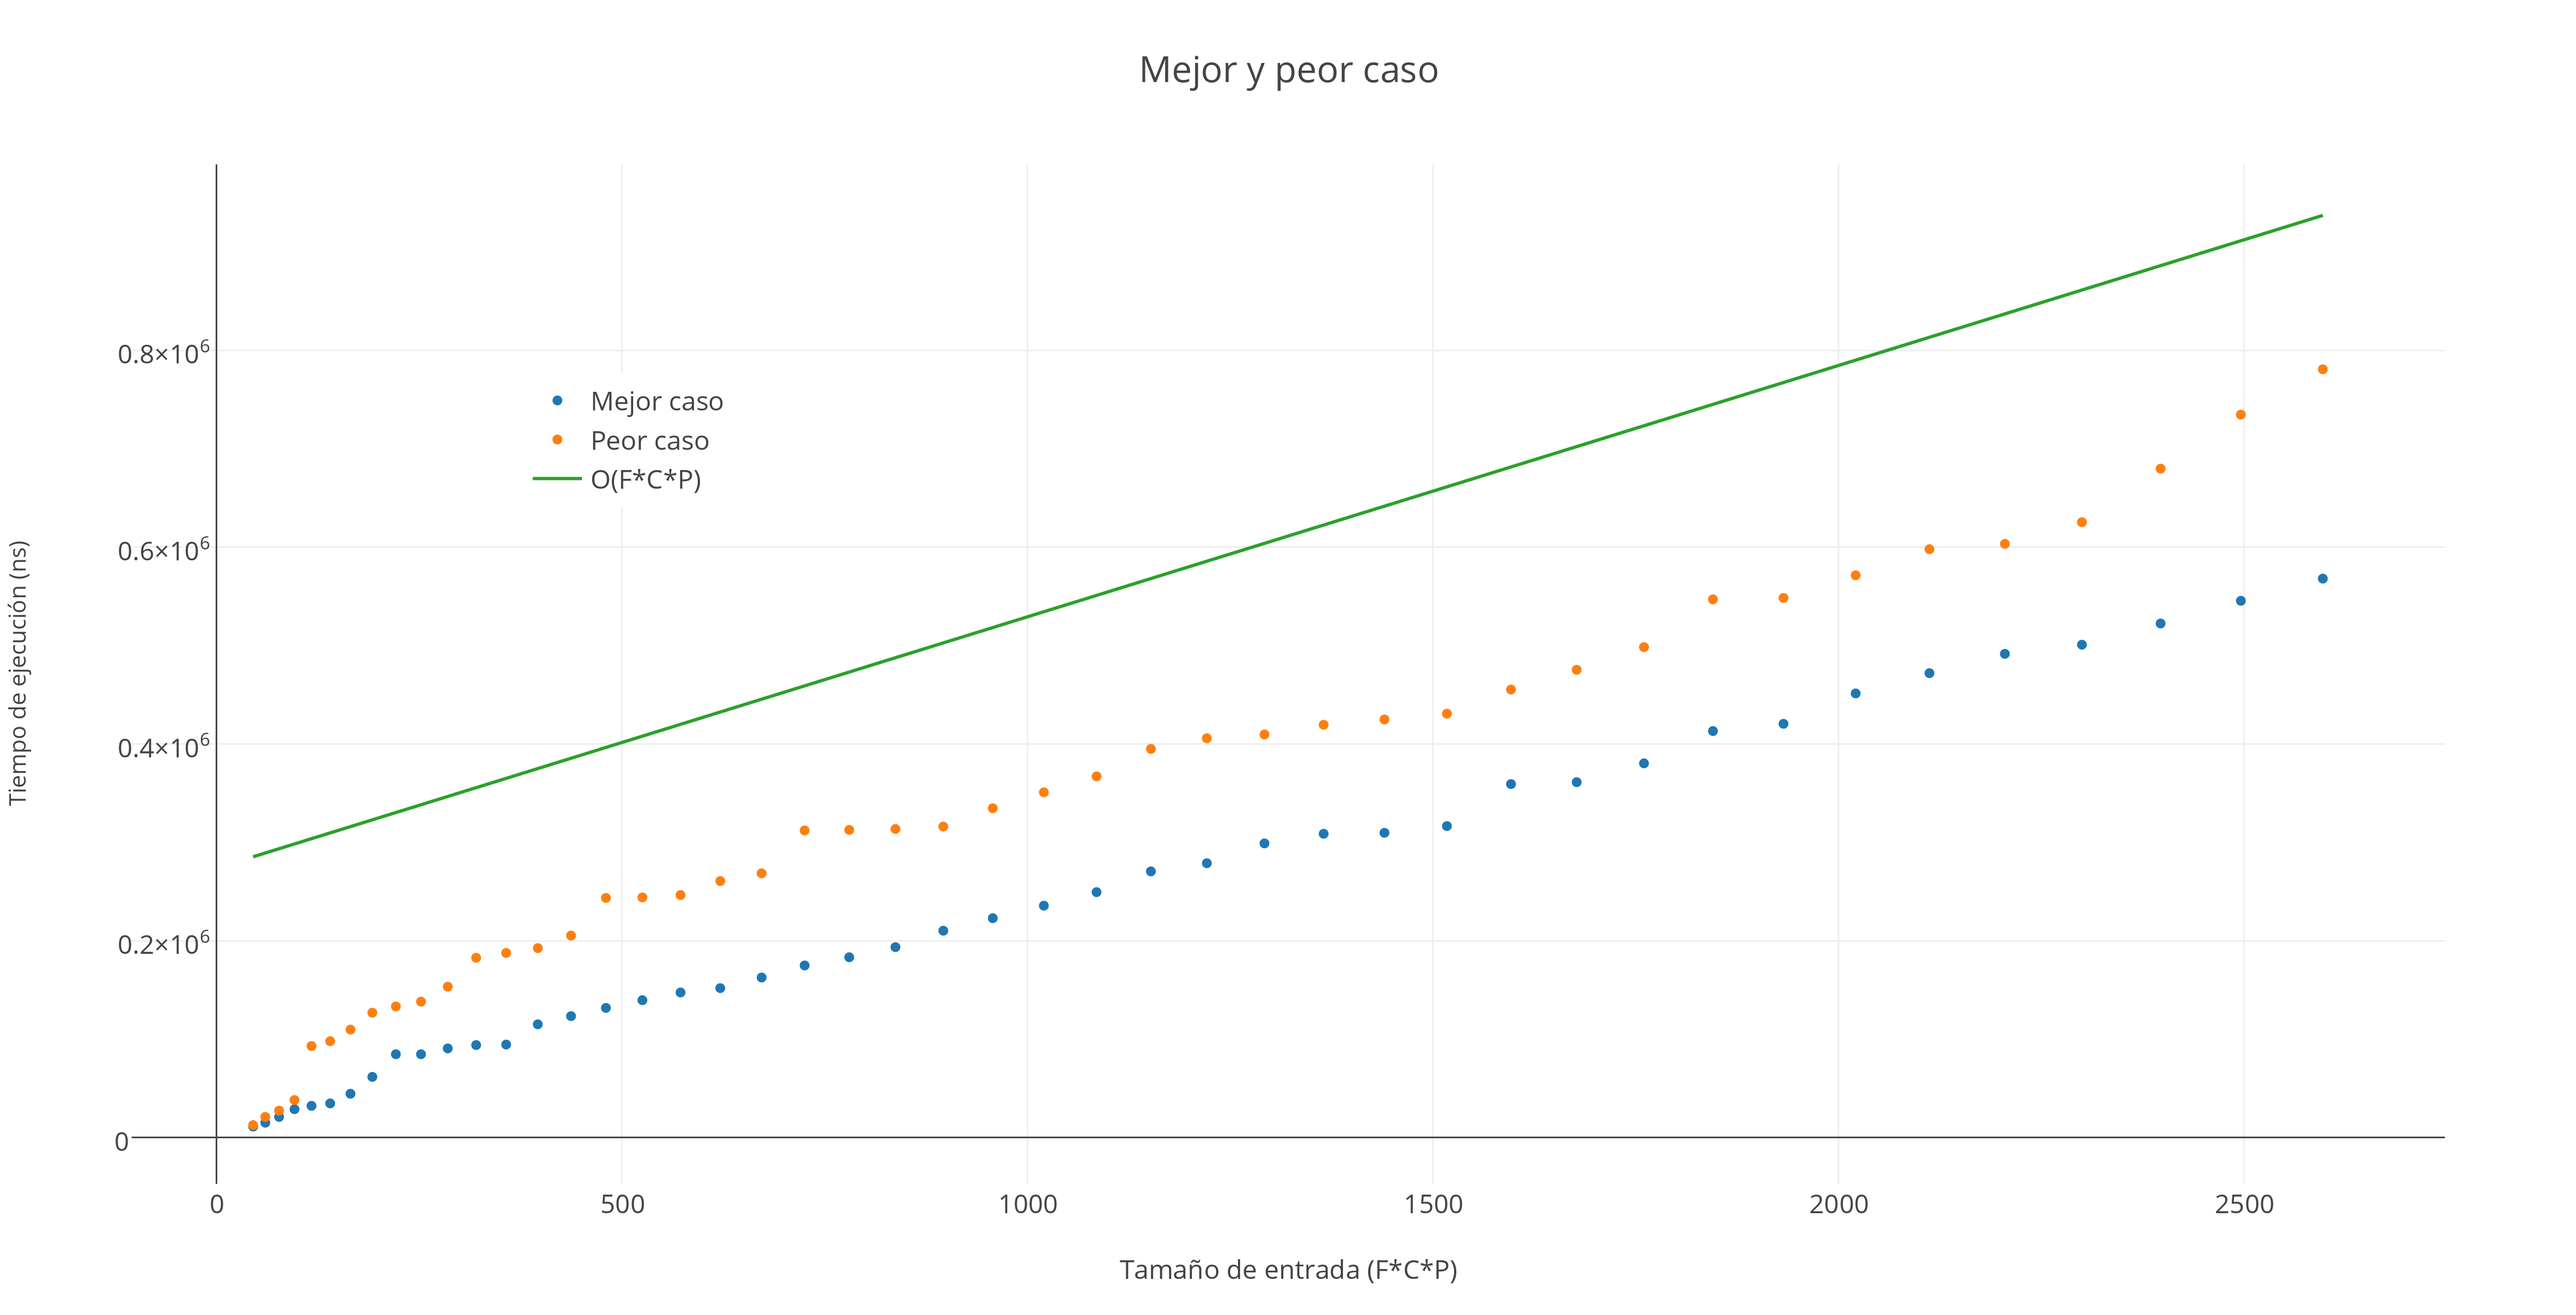
\includegraphics[scale=0.5]{./EJ1/MejorYPeorCaso.png}
{Gr\'afico 1.5 - $Comparativo$}
  \end{center}
  \vspace*{0.3cm}

EXPLICAR COMO SE OBTUVO EL FITEO CON LA COMPLEJIDAD!!!

Podemos ver en este gr\'afico comparativo como las familias est\'an acotadas por la funci\'on de la complejidad te\'orica calculada.\\

\subsubsection*{Variando $P_{max}$ en un laberinto}

Para el siguiente test vamos a trabajar con un laberinto de tamaño fijo, con el origen en la segunda columna y el destino en la penultima (misma fila), que además en cada posición solo tiene paredes. Siendo el laberinto de tamaño 100*100 habrá 96 paredes por fila (sin contar los bordes).
Mostraremos a continuaci\'on que sucede al variar $P_{max}$ desde 0 hasta 96.\\

\vspace*{0.3cm} \vspace*{0.3cm}
  \begin{center}
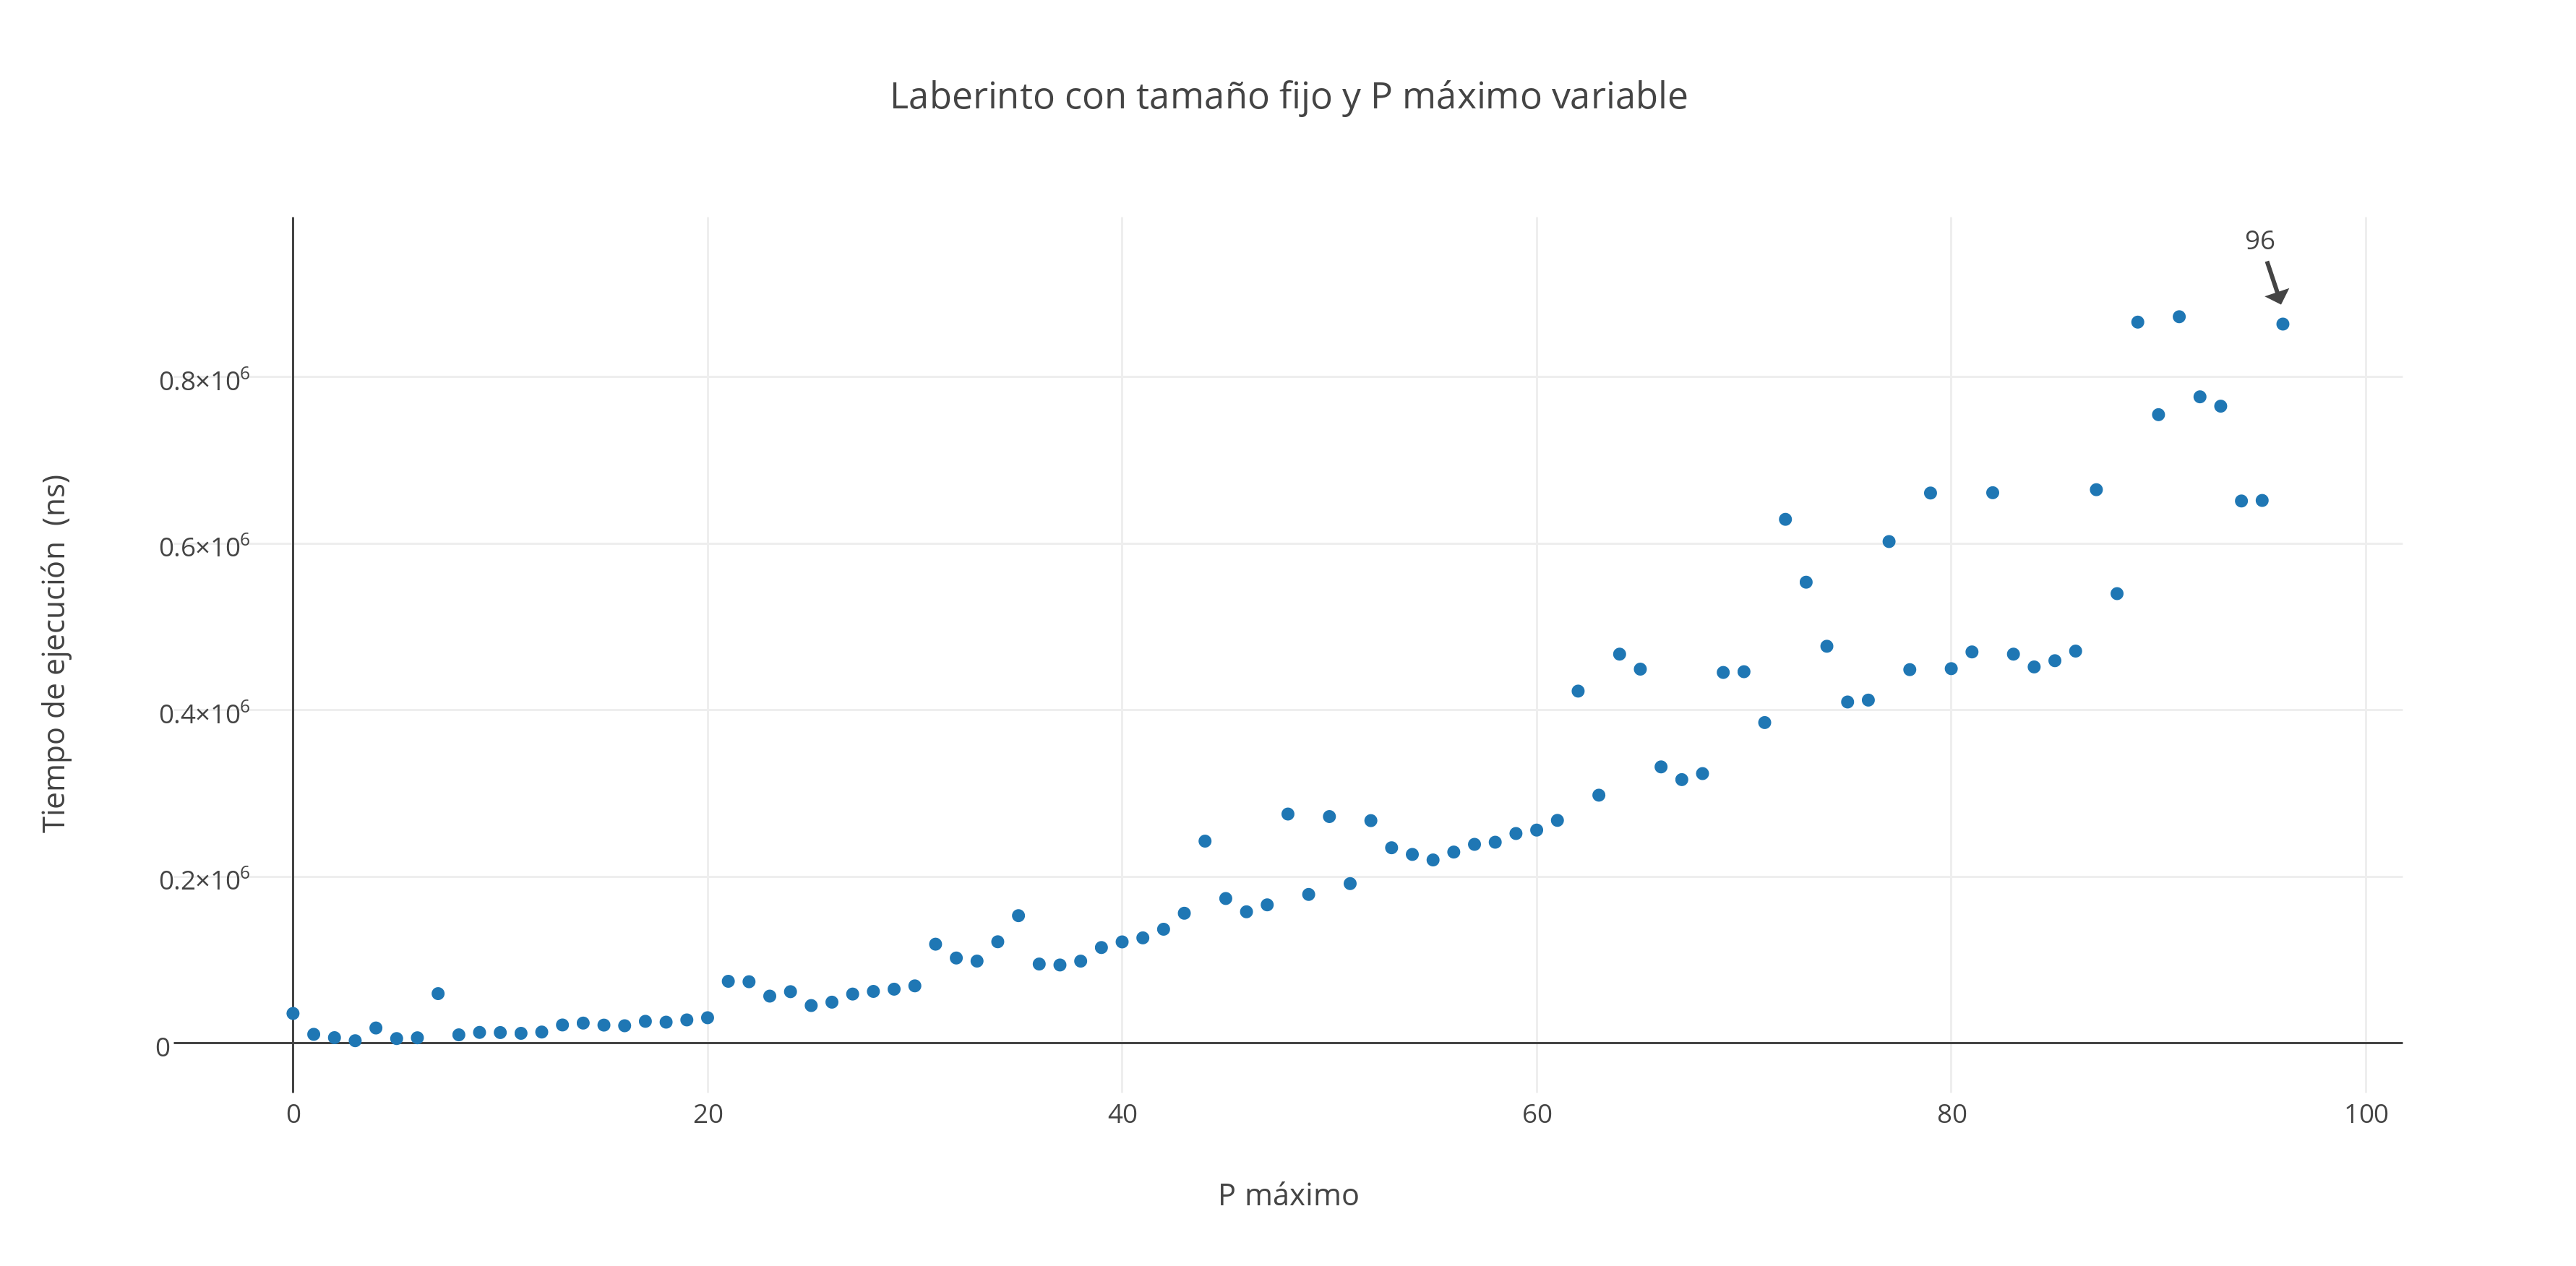
\includegraphics[scale=0.6]{./EJ1/pVariableBfs.png}
{Gr\'afico 1.6 - $P$ $variable$ $y$ $F,C$ $fijos$}
  \end{center}
  \vspace*{0.3cm}

Se puede observar en el gr\'afico 1.6 como al aumentar $P_{max}$, aumenta cuadráticamente el tiempo de resoluci\'on, ya que lo que sucede es que al aumentar el $P_{max}$ el algoritmo solo puede chequear en una sub matriz de $P_{max}^2$ caminos posibles a destino.\\
Al ser un algoritmo con espirutu $BFS$ recorre en anchura estas sub matrices, probando todas las posibilidades sin seguir un camino particular.  Por lo cual, que haya un camino directo a destino, rompiendo exactamente 96 paredes, no influye sobre el resultado. Ya que para llegar a destino, serán analizadas todas las posibilidades. 

Conociendo aproximadamente la dirección del mejor camino, si el algoritmo recorriera en profundidad (como un $DFS$), y además, el primer vecino analizado fuera el derecho (en dirección al destino), podría obtenerse un mejor resultado, ya que el camino elegido sería el directo al destino.\\ 
Por lo tanto fué modificado el algoritmo para utilizar una pila en lugar de una cola, y además apilar los vecinos de manera tal que el último en apilarse sea el derecho, obteniendo de esta manera un pseudo $DFS$ que nos permite corroborar este hecho.\\

  \begin{center}
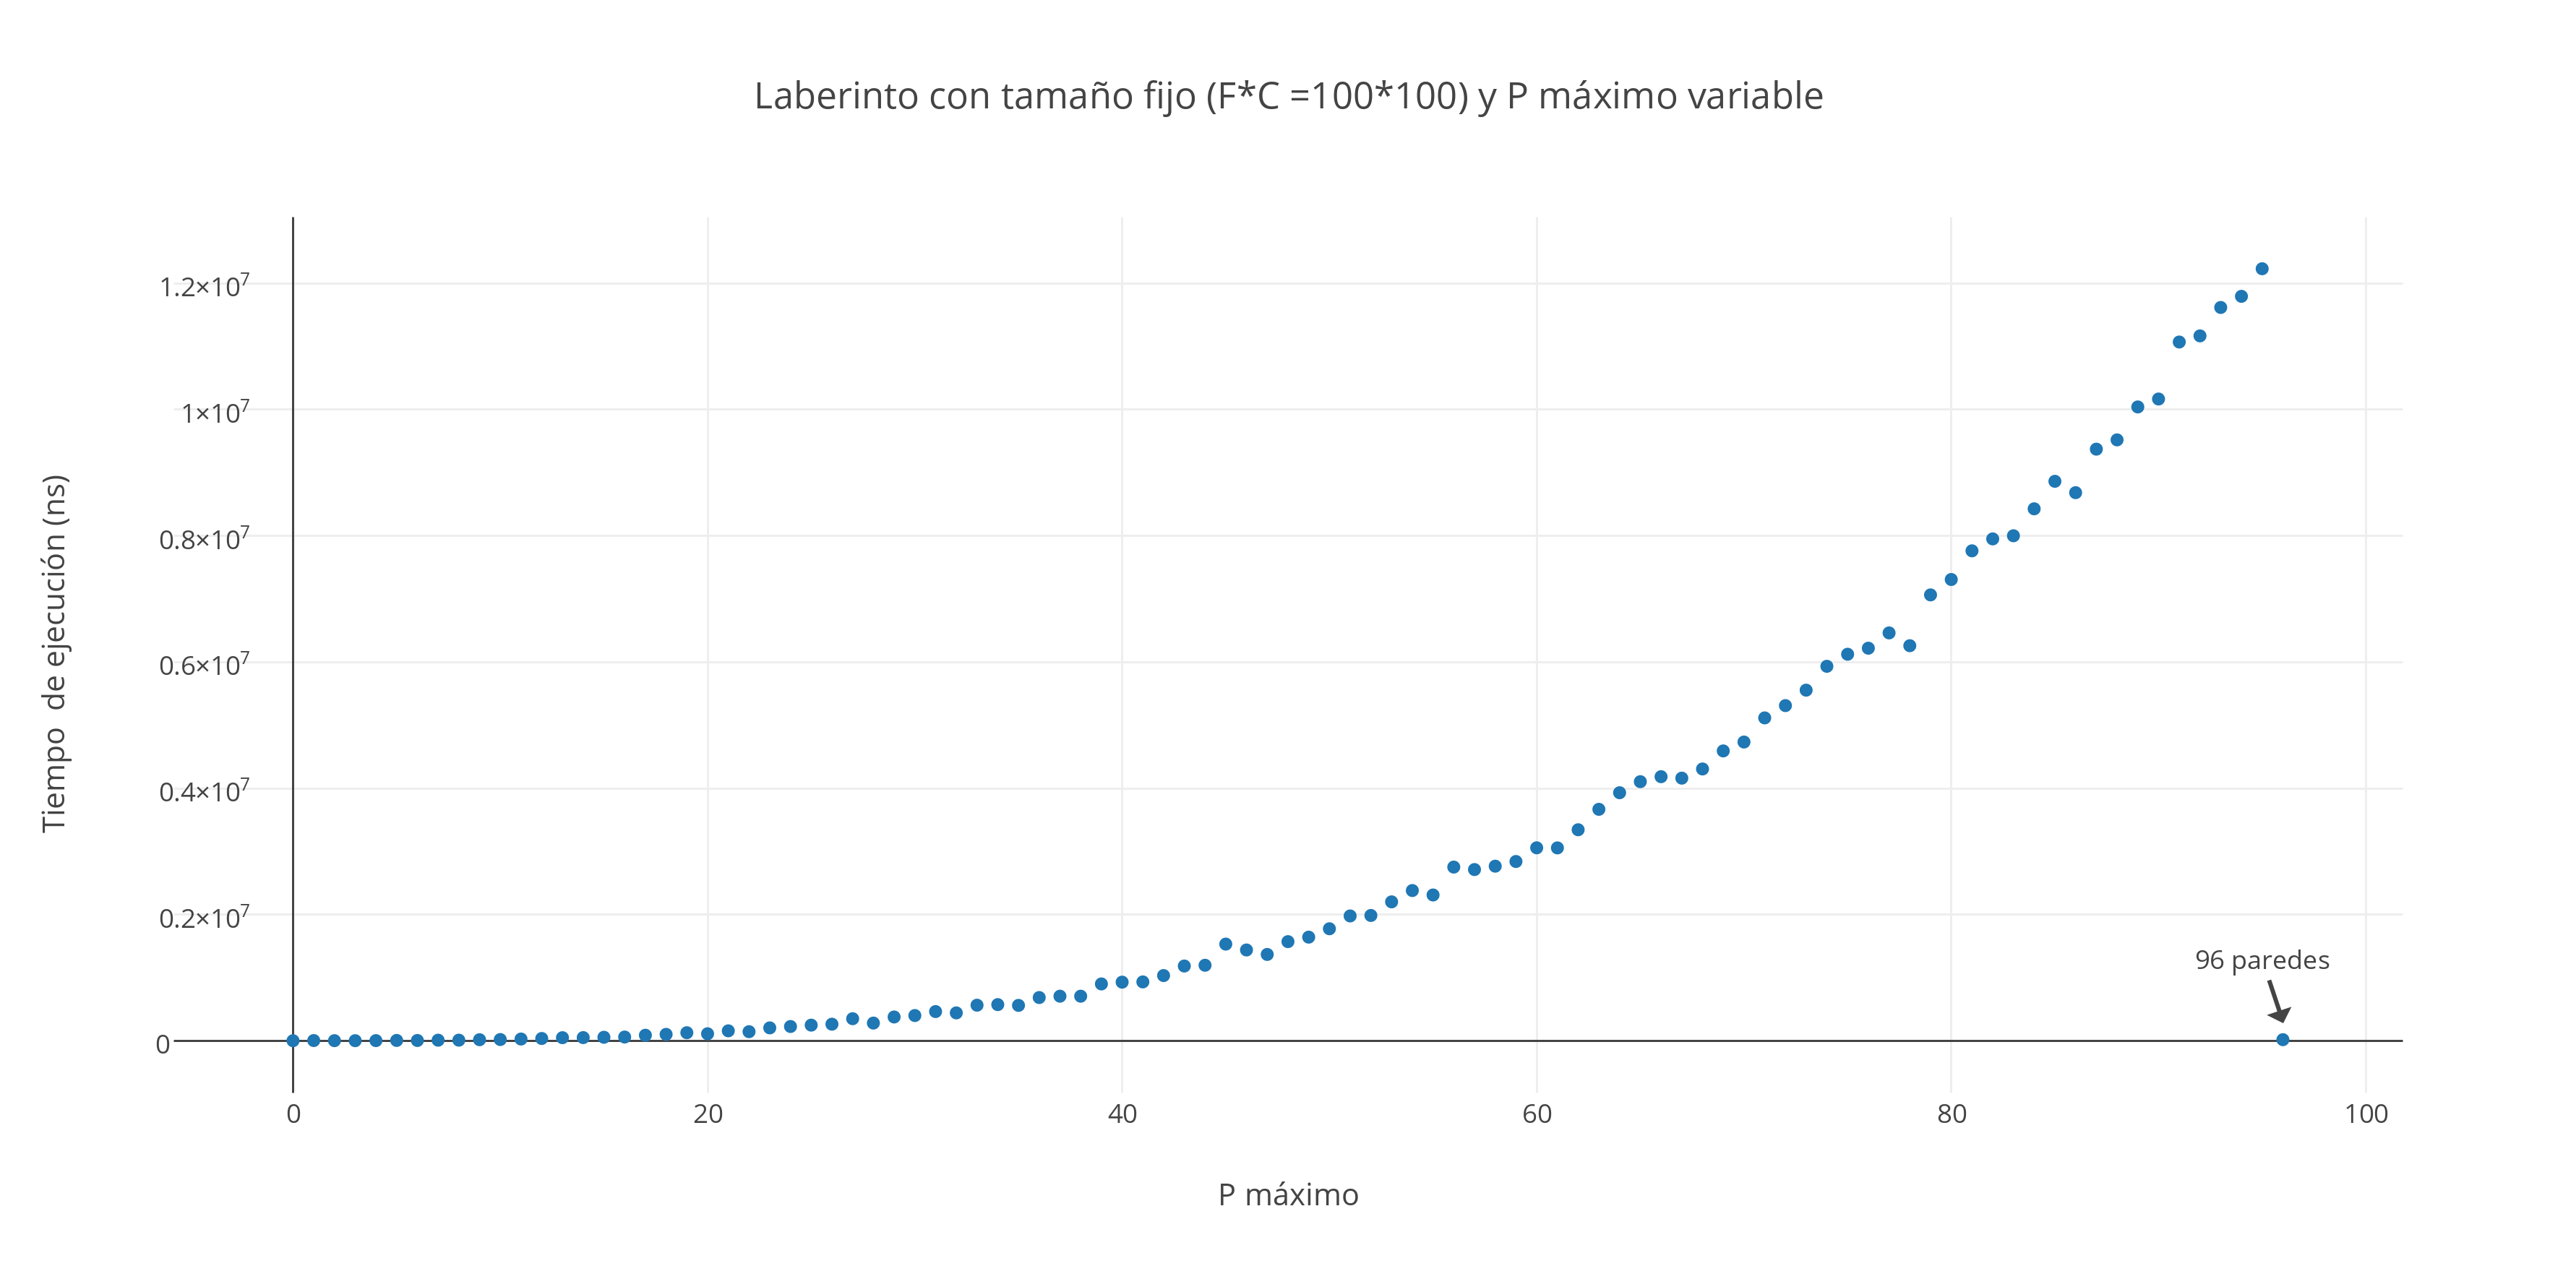
\includegraphics[scale=0.6]{./EJ1/pVariableDfs.png}
{Gr\'afico 1.7 - $P$ $variable$ $y$ $F,C$ $fijos$}
  \end{center}
  \vspace*{0.3cm}

Podemos observar en el gráfico 1.7 que el caso con $P_{max}$ = 96 hay solución, y se obtiene muy rapidamente debido a que el camino elegido es el directo a destino. Veamos que sucede en comparación al algoritmo original

  \begin{center}
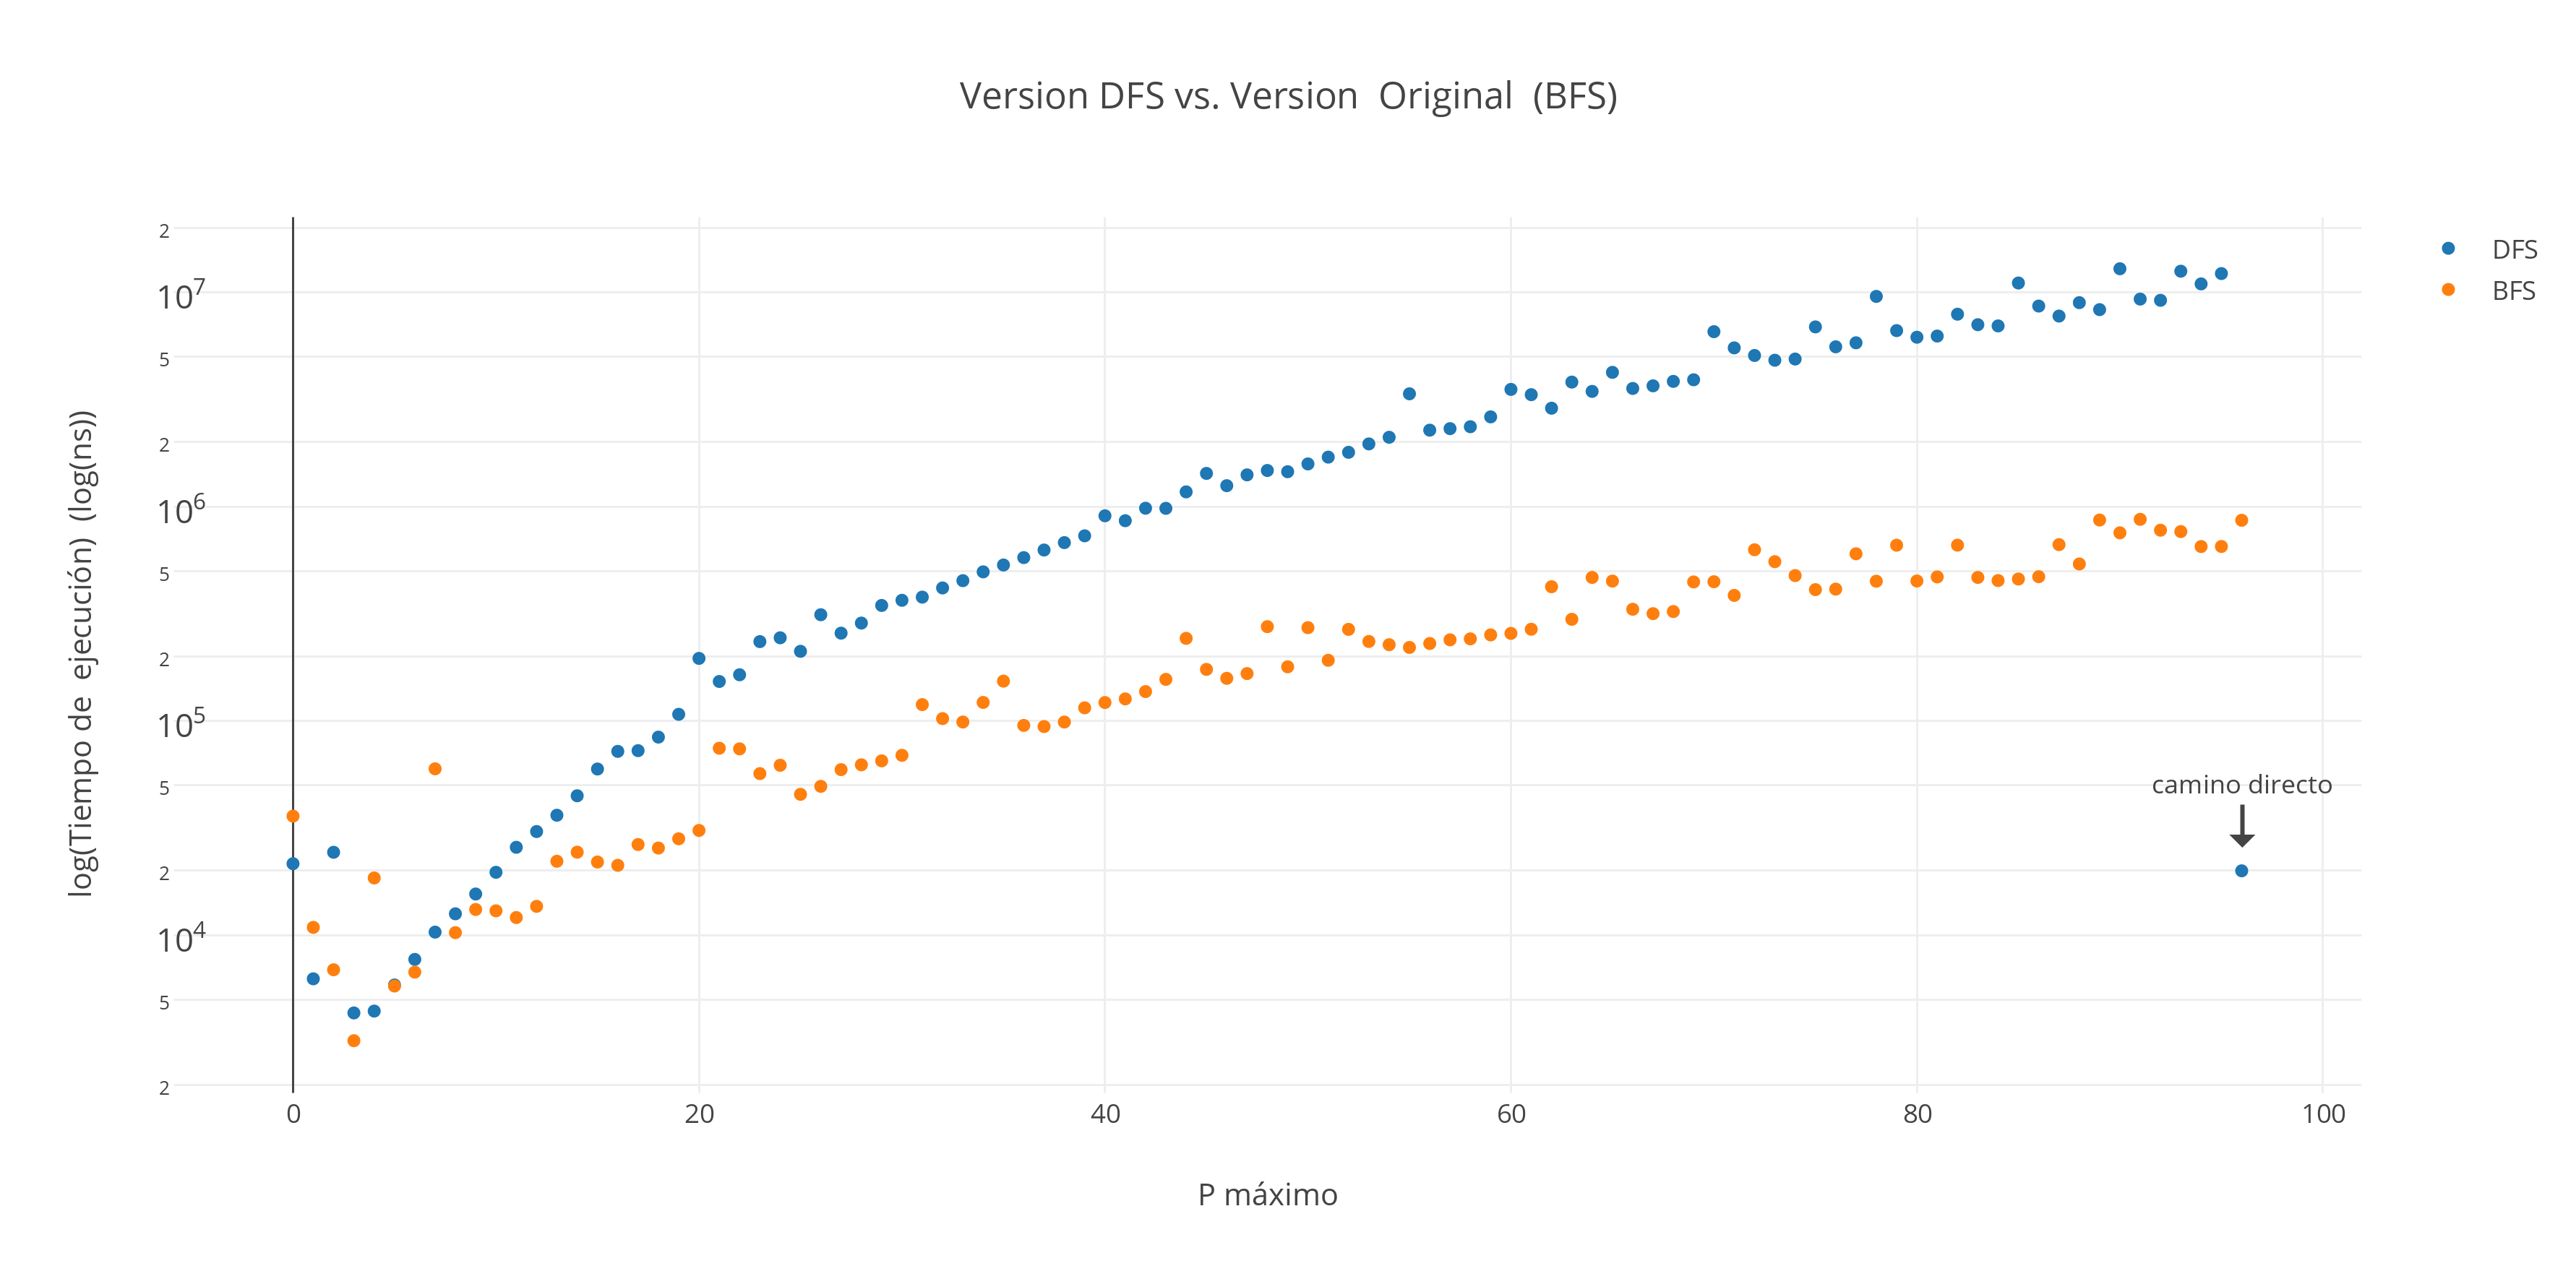
\includegraphics[scale=0.6]{./EJ1/bfsVsDfs.png}
{Gr\'afico 1.8 - $P$ $variable$ $y$ $F,C$ $fijos$}
  \end{center}
  \vspace*{0.3cm}
  
Podemos observar claramente, que bajo las condiciones planteadas para esta modificación, es un factor muy imporante saber en que dirección guiar la busqueda de este $DFS$. En el gráfico 1.8 podemos ver claramente como con $DFS$ se obtiene un resultado mucho mejor que el algoritmoo original ($BFS$). Concluyendo así lo supuesto al realizar los tests.

Luego de lo mostrado, se pudo observar que, tanto en el mejor como en el peor caso nuestro algoritmo se encuentra en el orden de la complejidad calculado y cumple con lo enunciado por el problema inicialmente. Además pudimos observar una particularidad del tipo de busqueda realizado y se propuso una variante al mismo que bajo ciertas condiciones puede mejorar el resultado original.
